\documentclass{article}
 
\usepackage[final, nonatbib]{nips_2017}

\usepackage[utf8]{inputenc} % allow utf-8 input
\usepackage[T1]{fontenc}    % use 8-bit T1 fonts
\usepackage{hyperref}       % hyperlinks
\usepackage{url}            % simple URL typesetting
\usepackage{booktabs}       % professional-quality tables
\usepackage{amsfonts}       % blackboard math symbols
\usepackage{nicefrac}       % compact symbols for 1/2, etc.
\usepackage{microtype}      % microtypography
\usepackage{bookmark}
\usepackage{graphicx}
\usepackage{svg}
\usepackage{verbatim}

\graphicspath{{images/}}
\svgpath{{images/}}

\title{Batch Normalization in Neural Networks Applied To Document Analysis}

\author{
  Andrew D.~Stelter \\
  Department of Computer Science\\
  South Dakota School of Mines and Technology\\
  Rapid City, SD, 57701 \\
  \texttt{andrew.stelter@mines.sdsmt.edu} \\
}

\begin{document}
% \nipsfinalcopy is no longer used

\maketitle

\begin{abstract}
  In the early 2000s, a number of papers were published outlining general practices for developing neural networks
  for image recognition. Since then, much research has gone into the field of neural networks and a number of general-purpose improvements have been found. We implemented one of the general-purpose neural network architectures and modified it to include one such recently-developed tool: batch normalization. By training this
  neural network on the MNIST training set we were able to show that the introduction of batch normalization yields better results for that application. Following the footsteps of the original paper implemented, we also tested this using expanded datasets produced by applying affine transformations and elastic deformations to the MNIST data.
\end{abstract}

\section{Introduction}

In the early 2000s, a Neural Nets were shown to be one of the best tools available for
document analysis and handwriting recognition. 
\cite{tay2001offline} \cite{sinha1999improved}
In their 2003 paper, Simard 
\cite{simard2003best} 
outlined a general-purpose neural net architecture that
is adequate for simple document analysis.

In their work, Simard achieved a 4\% error rate using a simple convolutional neural net to recognize digits from the MNIST 
\cite{mnist}
data set. Since the publishing of that paper, new general-purpose techniques have been developed which could be used to expand that architecture. In this paper, we compare that neural net's performance to the performance of one using one of those new techniques.

The technique in question is batch normalization as presented in 2015 by Sergey Ioffe and Christian Szegedy. 
\cite{ioffe2015batch}
Batch normalization can be used to accelerate the learning of neural nets by normalizing each batch of training data after each layer of the network. Doing this allows the gradients at each step to be independent of the data and gradients in other steps; this in turn allows the neurons of the neural net to learn at different rates.

We found that applying batch normalization to the network presented by Simard improves both the final scores and the number of epochs needed to train the neural net. While we did not achieve as low of an error rate, we were able to show this by comparing cases with our own neural net both using and ignoring batch normalization.

\section{Methods}
In the original paper by Simard, it is indicated that they developed the neural network from scratch. We made the decision to use one of the many neural network frameworks which has been put together since that paper. The framework which was chosen is Torch. 
\cite{torch}

Using Torch allowed rapid development of a neural network to process the MNIST database; in fact, the Torch project provides a neural net to do this as one of its example projects. While this example proved invaluable while learning how to use Torch, it did not follow the architecture laid out by Simard, so it was ultimately only useful for seeing how a Torch neural net program might be structured.

\subsection{Expanding the Dataset}
In their original paper, Simard outlines a number of methods used to expand the training dataset. They used both affine transformations and elastic deformations to created noisy and warped versions of the original images. The Torch Images library provides functionality for part of this process, thus we did not need to recreate the entire algorithm for applying affine transforms and elastic deformations to an image. We tested the neural net by producing four sets of training data:
\begin{itemize}
  \item The original MNIST dataset
  \item The original MNIST dataset and some transformed versions of each image
  \item The original MNIST dataset and some deformed versions of each image
  \item The original MNIST dataset and both transformed and deformed versions of each image
\end{itemize}

\subsubsection{Transforming the Images}
Simard does not outline the specific rules used to generate their affine transformations, so we picked a number of rules and used them to generate random 2x2 transformation matrices which could then be applied to the images. Each transform consisted of the following elements:
\begin{itemize}
  \item A random rotation in the range $\pm\frac{\pi}{16}$ radians
  \item A random shearing in both the x and y dimensions of $\pm 0.125$
  \item A random scaling in both the x and y dimensions of $\pm 0.25$
\end{itemize}

These are the ranges which were found to generate as much variance in the images as possible without changing them to the point of being unrecognizable. Some example transformations can be seen in Figure~\ref{fig:transforms}.

\begin{figure}
  \centering
  \includegraphics[width=0.15\textwidth]{original.png}
  \includegraphics[width=0.15\textwidth]{transform1.png}\\
  \includegraphics[width=0.15\textwidth]{transform2.png}
  \includegraphics[width=0.15\textwidth]{transform3.png}
  \caption{One of the original images (top left) and some examples of its affine tranformations}
  \label{fig:transforms}
\end{figure}

\subsubsection{Warping the Images}

As stated above, the Torch Images library provides much of the functionality needed to recreate the elastic deformations described by Simard. Their outline of the process described convolving two delta fields $\Delta x$ and $\Delta y$ with a gaussian of some standard deviation $\sigma$. The resulting displacement field could be scaled by some $\alpha$ and then applied to the original image to warp it.

Using the Torch Image library simplified this process greatly, and we were able to quickly start creating deformed data sets to test with. At the recommendation of Simard, we used $\sigma=4$ and $\alpha=34$; however, it is unknown whether or not the displacement fields produced through Torch were analogous to the ones produced by their algorithm. Some example vector fields and their resulting deformations can be seen in Figure~\ref{fig:deforms}.

\begin{figure}
  \centering
  \includegraphics[width=0.15\textwidth]{original.png}
  \includesvg[width=0.2\textwidth]{deform1.svg}
  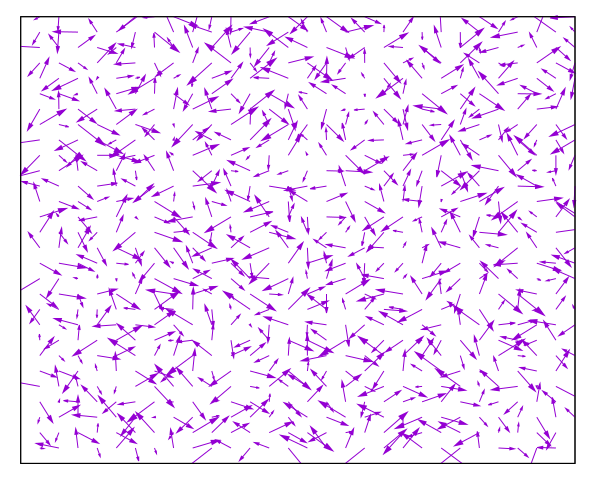
\includegraphics[width=0.15\textwidth]{deform1.png}\\
  \includesvg[width=0.2\textwidth]{deform2.svg}
  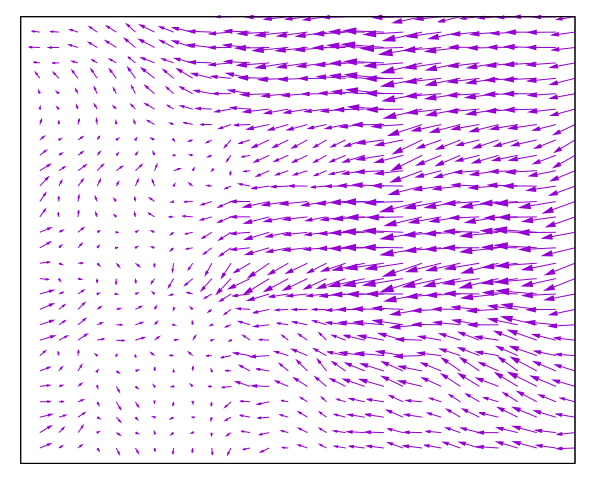
\includegraphics[width=0.15\textwidth]{deform2.png}
  \includesvg[width=0.2\textwidth]{deform3.svg}
  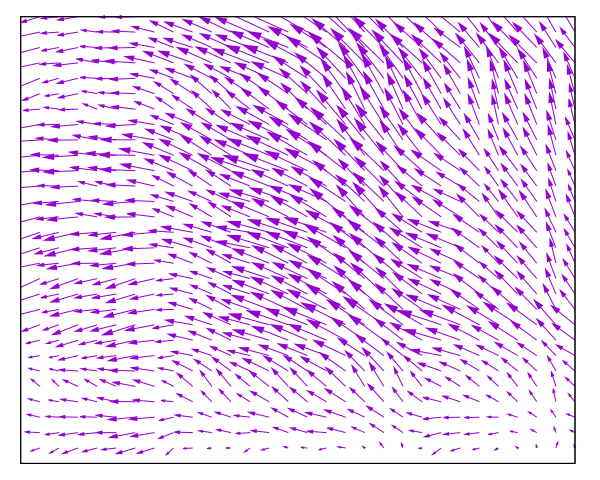
\includegraphics[width=0.15\textwidth]{deform3.png}
  \caption{One of the original images (top left) and vector fields with their resulting deformations. In order: $\sigma=0.001$, $\sigma=4$, and $\sigma=30$}
  \label{fig:deforms}
\end{figure}

\subsection{Network Architecture}
The network architecture outlined by Simard can be described succinctly as a feature extractor followed by a universal classifier. The feature extraction portion consisted of two spatial convolution layers, each having a kernel of size 5. This reduced the input image from 29x29 pixels to 5x5 pixels. The first layer of convolution output 5 planes size 13x13, and the second layer produced 50 planes. The universal classifier is described as two fully connected layers of neurons, sizes 100 and 10 respectively, with the layer of 10 being the output layer. The final error calculation was done using both Mean-Squared-Error and Cross-Entropy calculations.

Building the same neural net in Torch was fairly simple; however, a couple of minor changes had to be made in order to use the framework. The biggest difference was the connection between the feature extractor and the classifier. The feature extraction ended with a total of 1250 pixels in all of its planes combined, and in order to feed this data into the universal classifier, an extra fully connected layer of the same size had to be added between the extractor and the classifier. The second change was that we tested only with a cross-entropy error calculation; mean-squared-error was not tested in this project. Another change in the training was due to the fact that Simard did not note how many epochs were used to train their net, they only noted that they reduced the learning rate every 100 epochs. This indicates to us that they trained their net until it converged on a set of weights and stopped learning. Due to time and hardware constraints, we were not able to do that; however, preliminary tests indicated that, with our architecture, the most progress occured within the first 250 epochs, so we chose to end all training at that point. Finally, Simard does not note the transfer function used between the layers of his net. At the recommendation of the Torch quickstart tutorial \cite{torchTutorial} for identifying images in the CIFAR data set \cite{krizhevsky2009learning}, we used a ReLU transfer function between all layers of the neural net.

\subsection{Batch Normalization}
The main goal of this project was to determine how batch normalization as described by Ioffe and Szegedy would affect the network laid out by Simard. To this end, we made use of the Torch SpatialBatchNormalization and BatchNormalization layers after the convolution layers and linear layers, respectively. These layers were allowed to learn their $\beta$ and $\gamma$ parameters during training; the values were not taken from the dataset or provided as constants.

The power of batch normalization comes from training the neural net on small sets of the full training set known as minibatches. For each epoch trained, a random permutation of the full training set was generated, and then minibatches were made by taking sequential groups of $n$ items. Each minibatch was trained during that epoch as if it were a full training set. Picking minibatch sizes can be difficult and depends on the application of the neural net, so we tested our net using multiples of 100 up to 1000 which evenly divided the full training set size to see what yielded the best result.


\section{Results}
We varied four different factors across all our tests:
\begin{itemize}
\item Number of deformations of each image
\item Number of transformations of each image
\item Size of minibatch
\item Whether or not the batch normalization steps were used
\end{itemize}
The first two varibes were tied together - we tested using 10 deformations, 10 transformations, 5 of each, and 0 of each. Since we used multiples of 100 which divided the training and testing sets, we tested minibatches of sizes 100, 200, 400, 500, and 1000. These parameters led to a total of 40 cases to train and test the neural net on. An overview of the data collected can be seen in Tables \ref{table:nobatch} and \ref{table:batch}.

The best scoring test overall was 99.37\%. It was achieved using batch normalization with a batch size of 500 in conjunction with 10 deformations of each image of the data set. The worst score overall was 49.36\%, achieved with a minibatch size of 1000 on the original dataset.

\begin{table}[t]
  \caption{Highest Success Score of Each Neural Net without Batch Normalization}
  \centering
  \begin{tabular}{lllll}
    \toprule
    & Original Dataset & Only Deforms & Only Transforms & Deforms and Transforms \\
    \midrule
    Batch Size 100 & 98.65\% & 99.29\% & 98.90\% & 99.34\%  \\
    Batch Size 200 & 98.65\% & 99.28\% & 98.82\% &99.3\%  \\
    Batch Size 400 & 98.55\% & 99.32\% & 77.78\% & 99.30\%\\
    Batch Size 500 & 98.65\% & 89.5\% & 98.96\% & 99.32\% \\
    Batch Size 1000 & 49.36\% & 99.24\% & 98.88\% & 99.29\% \\
    \bottomrule
  \end{tabular}
  \label{table:nobatch}
\end{table}

\begin{table}[t]
  \caption{Highest Success Score of Each Neural Net with Batch Normalization}
  \centering
  \begin{tabular}{lllll}
    \toprule
    & Original Dataset & Only Deforms & Only Transforms & Deforms and Transforms \\
    \midrule
    Batch Size 100 & 98.88\% & 99.36\% & 99.15\% & 99.23\% \\
    Batch Size 200 & 98.92\% & 99.22\% & 99.07\% & 99.33\% \\
    Batch Size 400 & 98.83\% & 99.25\% & 99.1\% & 99.32\% \\
    Batch Size 500 & 98.72\% & 99.37\% & 99.1\% & 99.29\% \\
    Batch Size 1000 & 98.72\% & 99.30\% & 99.12\% & 99.25\% \\
    \bottomrule
  \end{tabular}
  \label{table:batch}
\end{table}

\subsection{Results of Extending the Data Set}
Extending the data set always resulted in smaller error. Including 10 deformations of each image reduced the error more than including just transforms and in most cases it also reduced the error more than including a combination of transforms and deforms. Figure \ref{fig:small-minibatch} shows the results of each test of the neural net using a minibatch size of 100, and Figure \ref{fig:large-minibatch} shows the same data for a minibatch size of 1000.

\begin{figure}
  \centering
  \includegraphics[width=0.75\textwidth]{Minibatch-Size---100.eps}
  \caption{Results of all training with minibatch size 100}
  \label{fig:small-minibatch}
\end{figure}
\begin{figure}
  \centering
  \includegraphics[width=0.75\textwidth]{Minibatch-Size---1000.eps}
  \caption{Results of all training with minibatch size 1000}
  \label{fig:large-minibatch}
\end{figure}

\subsection{Results of Normalization and Batch Size}
In general, smaller batch sizes performed better without batch normalization, but the introduction of batch normalization minimized this effect. More importantly, introducing the batch normalization step stabilized the learning rate and prevented large jumps along the gradient. In general, it also resulted in better testing scores than cases without it. Figures \ref{fig:base-compare} and \ref{fig:deform-compare} show side-by-side comparisons of the best and worst scoring tests. You can see that the neural nets training on the original data set performed better when the batch normalization steps were introduced, and you can also see that smaller minibatches performed better when batch normalization was not used.

\begin{figure}
  \centering
  \includegraphics[width=0.75\textwidth]{Base-Data---No-Batch-Normalize.eps}
  \includegraphics[width=0.75\textwidth]{Base-Data---Batch-Normalized.eps}
  
  \caption{Graphs of results for all minibatch sizes for the original data set with (left) and without(right) batch normalization}
  \label{fig:base-compare}
\end{figure}

\begin{figure}
  \centering
  \includegraphics[width=0.75\textwidth]{Deforms---No-Batch-Normalize.eps}
  \includegraphics[width=0.75\textwidth]{Deforms---Batch-Normalized.eps}

  \caption{Graphs of results for all minibatch sizes for the dataset extended by elastic deformation with (left) and without(right) batch normalization}
  \label{fig:deform-compare}
\end{figure}

\section{Conclusions}
We found that, while the general-purpose architecture proposed by Simard is effective by itself, it can be improved upon by using newly discovered techniques. The technique tested was that of Batch Normalization, as defined by Ioffe and Szegedy. As can be seen in figures \ref{fig:base-compare} and \ref{fig:deform-compare}, including a batch normalize step after each stage of the neural net produced two measurable results:
\begin{itemize}
  \item The neural net reached a high score with fewer epochs because the gradient decent was able to learn more consistently
  \item The nerual net scored higher overall when tested
\end{itemize}

In their original paper, Simard recorded that they achieved the highest score on MNist at the time: 0.4\% error. We were not able to match that score; however, we did get very close with 0.64\% error. There are a number of differences between the projects that may account for this difference. First of all, Simard produced their neural net from scratch; we used the Torch framework. This difference alone could be considered enough to cause the discrepancy, as we don't know what the difference between the executed code was. Similarly, we used the Torch libraries for image manipulation, and Simard presumably wrote their own routines to transform and warp images; this may have resulted in sub-optimal deformations, as we used the $\sigma$ and $\alpha$ values that were found to work best for Simard. We believe the next difference is that we did not train our nets as long. Simard noted that they "used  a  learning  rate  that  
started  at  0.005  and  [was]  multiplied  by  0.3  every  100  
epochs." This implies that they trained their net for multiple hundreds of epochs. Due to time and hardware constraints, we were only able to train our nets for 250 epochs each. Reducing the learning rate over time and training longer may have produced better results. Additionally, Simard does not note how many deformed copies of the data set were used; creating more warped versions of each image may also have resulted in a lower error for our neural net.
\section{References}
\bibliographystyle{IEEEtran}
\bibliography{sources}

\end{document}
